\chapter{Statistical Distributions for Financial Asset Prices and Returns}
\label{chap:Statistical Distributions for Financial Asset Prices and Returns}

\begin{center}
\begin{tabular}{p{0.06\linewidth} | p{0.88\linewidth}}
	\toprule
	\multicolumn{2}{l}{\textbf{LEARNING OUTCOMES}} \\
	\midrule
	a & calculate, interpret, and evaluate unconditional expected values for mean, variance, and covariance \\
	\midrule
	b & calculate, interpret, and evaluate the principal moments of key statistical distributions used in finance \\
	\midrule
	c & calculate, interpret, and evaluate conditional expectations, variances, and covariances \\
	\midrule
	d & formulate investment problems through Bayesian updating \\
	\bottomrule
\end{tabular}
\end{center}

\vspace{1.5em}

\begin{itemize}
	\item[] \textbf{Random Variables and Unconditional Expectations}
	      \begin{itemize}
			\item[] Random Variables and Their Properties
			\item[] Unconditional Expectations, Variance, and Covariance
		  \end{itemize}
	\item[] \textbf{Key Statistical Distributions in Finance}
	      \begin{itemize}
			\item[] Discrete Statistical Distributions
			\item[] Continuous Statistical Distributions
			\item[] Practical Implementation
		  \end{itemize}
	\item[] \textbf{Conditional Expectations, Variances, and Covariances}
	      \begin{itemize}
			\item[] Joint Distributions of Random Variables
			\item[] Conditional Expectations
			\item[] Conditional Means, Variances, and Covariances
	      \end{itemize}
	\item[] \textbf{Bayesian Updating}
\end{itemize}

% \textcolor{blue}{\textit{Mục tiêu Module 6: hiểu cách dùng các phân phối (Nhị thức, Poisson, Chuẩn, Log-normal) để mô hình hóa giá, sinh lời và rủi ro. Đặc biệt lưu ý định lý Bayes vì tần suất xuất hiện cao.}}

% \textcolor{blue}{\textit{Lộ trình học: (1) Xác suất biến liên tục là diện tích dưới đường cong PDF (không cần tính tích phân). (2) Tập trung vào biến rời rạc và định lý Bayes. (3) Ghi nhớ 4 moments của các phân phối và lý do lựa chọn (Log-normal cho giá $\ge 0$, Poisson cho số vụ vỡ nợ).}}

\section{Random Variables and Unconditional Expectations}
\label{sec:Random Variables and Unconditional Expectations}
\begin{center}
\begin{tabular}{p{0.06\linewidth} | p{0.88\linewidth}}
	a & calculate, interpret, and evaluate unconditional expected values for mean, variance, and covariance \\
\end{tabular}
\end{center}

\subsection{Random Variables and Their Properties}
	\label{subsec:Random Variables and Their Properties}
A \textbf{random variable} is a function that assigns a number to each outcome of an experiment. In finance, random variables are often called \textbf{stochastic variables}, reflecting their inherent unpredictable nature. Random variables are categorized into two types:
\begin{itemize}
	\item A \textbf{discrete random variable} has a countable number of distinct outcomes. For example, a fair coin toss results in heads or tails, each with a probability of $p = 0.50$. Similarly, rolling a fair six-sided die yields outcomes of $1, 2, 3, 4, 5,$ or $6$, each with a probability of $p = \frac{1}{6}$.
	\item A \textbf{continuous random variable} can take on an infinite number of possible values within a given range, such as picking a random number between $0$ and $1$ on the number line. When the number of observations is large, empirical distributions often converge to continuous distributions.
\end{itemize}

\textcolor{blue}{\textit{Biến rời rạc (Discrete) mô tả các sự kiện đếm được (số vụ vỡ nợ, giao dịch). Tỷ suất sinh lời cổ phiếu dùng biến liên tục (Continuous) vì có thể nhận bất kỳ giá trị thực nào.}}

A random variable, $X$, is fully described by its distribution functions:
\begin{figure}[!htbp]
	\centering
	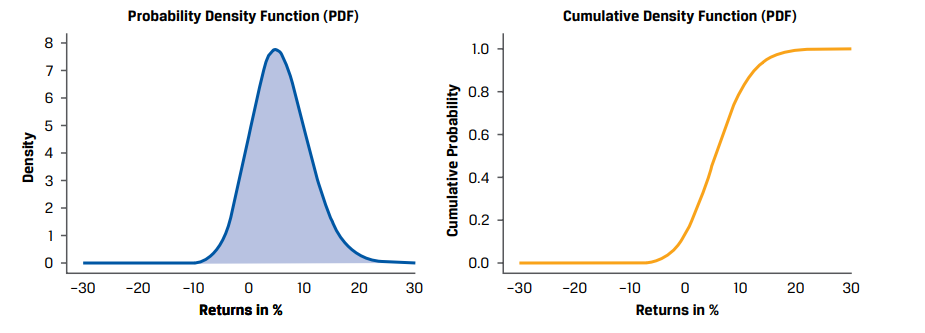
\includegraphics[width=0.85\linewidth]{002_figs/006_Module_6/exhibit_3.png}
	\caption{Theoretical PDF and CDF of Daily Stock Returns}
	\label{fig:mod6_exhibit_3}
\end{figure}

\begin{figure}[!htbp]
	\centering
	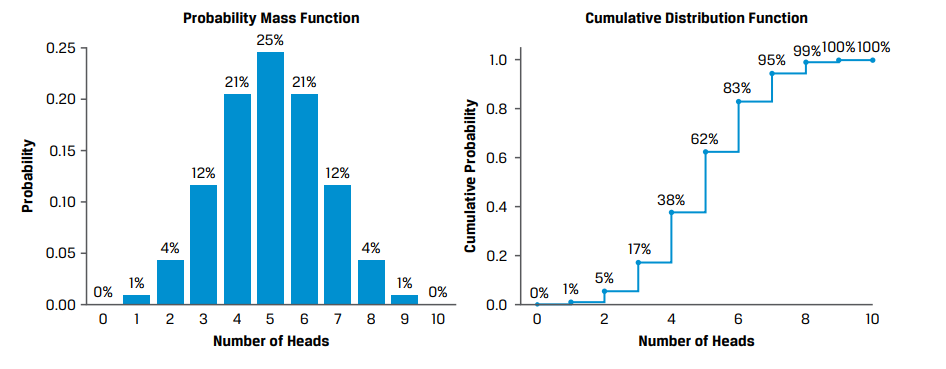
\includegraphics[width=0.85\linewidth]{002_figs/006_Module_6/exhibit_4.png}
	\caption{The PMF and CDF of the Coin Toss Experiment}
	\label{fig:mod6_exhibit_4}
\end{figure}

\begin{itemize}
	\item \textbf{Cumulative Distribution Function (CDF):} Gives the probability that the random variable $X$ takes on a value less than or equal to $x$:
	\begin{equation}
		F(x) = P(X \le x)
		\label{eq:cdf_def_m6}
	\end{equation}
	The CDF is non-decreasing with $\lim_{x \to -\infty} F(x) = 0$ and $\lim_{x \to \infty} F(x) = 1$. The CDF applies to both discrete and continuous random variables.
	
	% \textcolor{blue}{\textit{Giải thích trực quan: CDF $F(x)$ cho biết xác suất để biến ngẫu nhiên $X$ nhận giá trị nhỏ hơn hoặc bằng một mốc $x$ cho trước. Ví dụ, đối với tỷ suất sinh lời của cổ phiếu, $F(5\%) = 0.85$ nghĩa là có $85\%$ khả năng tỷ suất sinh lời thực tế sẽ không vượt quá $5\%$. Vì là xác suất lũy kế, CDF luôn tăng (hoặc giữ nguyên) từ $0$ (tại $-\infty$) đến $1$ (tại $+\infty$).}}

	\item \textbf{Probability Density Function (PDF):} For continuous random variables, the PDF is the derivative of the CDF, representing the instantaneous rate of change of the CDF:
	\begin{equation}
		f_X(x) = \frac{dF_X(x)}{dx}
		\label{eq:pdf_derivative_m6}
	\end{equation}
	The probability that $X$ falls within an interval $[a, b]$ is the area under the PDF curve between $a$ and $b$:
	\begin{equation}
		P(a \le X \le b) = \int_a^b f_X(x) dx = F(b) - F(a)
		\label{eq:pdf_probability_interval_m6}
	\end{equation}
	The total area under the PDF curve equals $1$:
	\begin{equation}
		\int_{-\infty}^{\infty} f_X(x) dx = 1
		\label{eq:pdf_total_area_m6}
	\end{equation}
	
	% \textcolor{blue}{\textit{Giải thích trực quan: Đối với biến ngẫu nhiên liên tục (như tỷ suất sinh lời), xác suất tại một điểm chính xác bằng $0$ (tức là $P(X = 5.0000\%) = 0$). Do đó, ta không dùng xác suất tại một điểm mà dùng hàm mật độ PDF. Xác suất để biến số rơi vào một khoảng $[a, b]$ chính là diện tích nằm dưới đường cong PDF giới hạn bởi hai đầu mút $a$ và $b$ này.}}

	\item \textbf{Probability Mass Function (PMF):} For discrete random variables, the PMF gives the probability that $X$ is exactly equal to a specific value $x$, $P(X=x)$. The probability that $X$ lies within $[a, b]$ is:
	\begin{equation}
		P(a \le X \le b) = \sum_{x=a}^b P(X=x)
		\label{eq:pmf_probability_interval_m6}
	\end{equation}
	The sum of probabilities for all possible outcomes equals $1$: $\sum_x P(X=x) = 1$.
	
	% \textcolor{blue}{\textit{Giải thích trực quan: PMF là hàm tính xác suất trực tiếp cho biến ngẫu nhiên rời rạc (đếm được). Khác với biến liên tục, ở đây ta có thể tính chính xác xác suất tại một điểm. Ví dụ, xác suất gieo xúc xắc được mặt $6$ chấm là $P(X=6) = \frac{1}{6}$. Tổng xác suất của mọi kết quả có thể xảy ra luôn bằng $1$.}}
\end{itemize}

\begin{figure}[!htbp]
	\centering
	\begin{subfigure}[b]{0.48\linewidth}
		\centering
		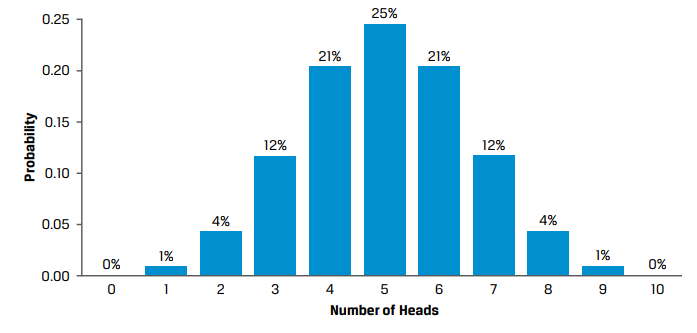
\includegraphics[width=\linewidth]{002_figs/006_Module_6/exhibit_1.png}
		\caption{Discrete PMF (Coin Tosses)}
		\label{fig:mod6_exhibit_1}
	\end{subfigure}
	\hfill
	\begin{subfigure}[b]{0.48\linewidth}
		\centering
		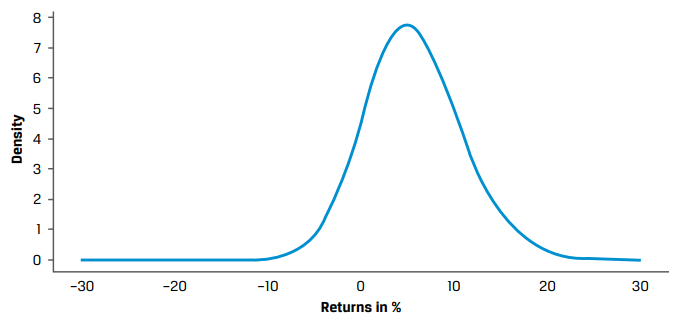
\includegraphics[width=\linewidth]{002_figs/006_Module_6/exhibit_2.png}
		\caption{Continuous PDF (Stock Returns)}
		\label{fig:mod6_exhibit_2}
	\end{subfigure}
	\caption{Discrete vs. Continuous Probability Distributions}
	\label{fig:discrete_vs_continuous_m6}
\end{figure}

\subsection{Unconditional Expectations, Variance, and Covariance}
	\label{subsec:Unconditional Expectations, Variance, and Covariance}
Unconditional expectations, variance, and covariance provide foundational tools for assessing the behavior of financial assets without requiring prior knowledge of specific market conditions.
\begin{itemize}
	\item \textbf{Unconditional Mean (Expected Value):} The probability-weighted average of the outcomes of a random variable over an infinite number of trials:
	\begin{equation}
		\text{Discrete: } \mu_X = E[X] = \sum_i x_i P(x_i)
		\label{eq:discrete_expected_value_m6}
	\end{equation}
	\begin{equation}
		\text{Continuous: } \mu_X = E[X] = \int_{-\infty}^{\infty} x f_X(x) dx
		\label{eq:continuous_expected_value_m6}
	\end{equation}
	
	% \textcolor{blue}{\textit{Giải thích trực quan: Kỳ vọng $E[X]$ (hay giá trị trung bình tổng thể $\mu$) là thước đo xu hướng trung tâm của phân phối. Đối với biến rời rạc, nó là trung bình trọng số của các kết quả có thể xảy ra với trọng số là xác suất tương ứng. Đối với biến liên tục, nó được tính bằng tích phân của giá trị biến số nhân với mật độ xác suất tương ứng.}}

	\item \textbf{Unconditional Variance:} Measures the squared dispersion of a random variable around its mean:
	\begin{equation}
		\sigma_X^2 = \text{Var}(X) = E[(X - E[X])^2] = E[X^2] - (E[X])^2
		\label{eq:unconditional_variance_m6}
	\end{equation}
	
	\textcolor{blue}{\textit{Phương sai $\text{Var}(X)$ (hay $\sigma^2$) đo lường mức độ biến động hoặc rủi ro của tài sản. Phương sai càng lớn nghĩa là giá trị thực tế càng dễ phân tán xa khỏi trung bình, đồng nghĩa với rủi ro càng cao.}}

	\item \textbf{Unconditional Standard Deviation:} $\sigma_X = \sqrt{\text{Var}(X)}$.
	
	\textcolor{blue}{\textit{Độ lệch chuẩn đưa thước đo biến động về cùng đơn vị đo với biến gốc, giúp dễ so sánh trực tiếp.}}

	\item \textbf{Unconditional Covariance:} Quantifies the linear relationship between two random variables $X$ and $Y$:
	\begin{equation}
		\sigma_{XY} = \text{Cov}(X, Y) = E[(X - E[X])(Y - E[Y])] = E[XY] - E[X]E[Y]
		\label{eq:unconditional_covariance_m6}
	\end{equation}
\end{itemize}

% \begin{tcolorbox}[
% 	colback=gray!5!white,
% 	colframe=black!15!white,
% 	boxrule=0.5pt,
% 	arc=3pt,
% 	title=\textbf{Case Study: Expected Mean, Variance, and Covariances of Two Dice},
% 	coltitle=black,
% 	colbacktitle=black!5!white,
% 	before skip=6pt,
% 	after skip=6pt,
% 	breakable
% ]
% For two fair dice, the expected sum is:
% \[ E[X] = 2\left(\frac{1}{36}\right) + 3\left(\frac{2}{36}\right) + \dots + 12\left(\frac{1}{36}\right) = 7 \]
% To calculate variance, we find the expected value of $X^2$:
% \[ E[X^2] = 2^2\left(\frac{1}{36}\right) + 3^2\left(\frac{2}{36}\right) + \dots + 12^2\left(\frac{1}{36}\right) = 54.84 \]
% \[ \text{Var}(X) = E[X^2] - (E[X])^2 = 54.84 - 7^2 = 5.84 \]
% Since rolls are independent, the covariance between the two individual dice is:
% \[ \text{Cov}(X, Y) = E[XY] - E[X]E[Y] = 12.25 - (3.5 \times 3.5) = 0 \]
% \end{tcolorbox}

\begin{tcolorbox}[
	colback=gray!5!white,
	colframe=black!15!white,
	boxrule=0.5pt,
	arc=3pt,
	title=\textbf{Case Study: Unconditional Mean, Variance, and Covariances of Two Assets},
	coltitle=black,
	colbacktitle=black!5!white,
	before skip=6pt,
	after skip=6pt,
	breakable
]
An analyst forecasts the performance of a stock index ($X$) and a bond index ($Y$) under different conditions:
\begin{center}
\begin{tabular}{c c c}
\toprule
\textbf{Probability} $P$ & \textbf{Stock Return} $X$ (\%) & \textbf{Bond Return} $Y$ (\%) \\
\midrule
0.2 & $-2.00$ & $0.75$ \\
0.3 & $-1.00$ & $0.50$ \\
0.3 & $0.00$  & $0.25$ \\
0.2 & $1.00$  & $0.00$ \\
\bottomrule
\end{tabular}
\end{center}
Calculating expectations:
\begin{align*}
	E[X] &= (-2.00 \times 0.2) + (-1.00 \times 0.3) + (0 \times 0.3) + (1.00 \times 0.2) = -0.50\% \\
	E[Y] &= (0.75 \times 0.2) + (0.50 \times 0.3) + (0.25 \times 0.3) + (0 \times 0.2) = 0.375\%
\end{align*}
Calculating variance:
\begin{align*}
	E[X^2] &= (0.2 \times (-2)^2) + (0.3 \times (-1)^2) + (0.3 \times 0^2) + (0.2 \times 1^2) = 1.30 \\
	\text{Var}(X) &= 1.30 - (-0.50)^2 = 1.05 \implies \sigma_X = \sqrt{1.05} = 1.025\% \\
	E[Y^2] &= (0.2 \times 0.75^2) + (0.3 \times 0.50^2) + (0.3 \times 0.25^2) + 0 = 0.2063 \\
	\text{Var}(Y) &= 0.2063 - 0.375^2 = 0.0656 \implies \sigma_Y = \sqrt{0.0656} = 0.2562\%
\end{align*}
Calculating covariance:
\begin{align*}
	E[XY] &= (0.2 \times (-2 \times 0.75)) + (0.3 \times (-1 \times 0.50)) + 0 + 0 = -0.45 \\
	\text{Cov}(X, Y) &= E[XY] - E[X]E[Y] = -0.45 - (-0.50 \times 0.375) = -0.2625
\end{align*}
The negative covariance of $-0.2625$ indicates that stocks and bonds tend to move in opposite directions, providing significant diversification benefits for a portfolio.
\end{tcolorbox}

\subsection{The Law of Large Numbers (LLN)}
	\label{subsec:The Law of Large Numbers (LLN)}
The \textbf{Law of Large Numbers} states that as the number of trials (sample size) increases, the empirical sample mean converges to the true population parameter (unconditional mean), assuming the sample is randomly drawn and representative of the population.

% \textcolor{blue}{\textit{Định luật số lớn (LLN) đảm bảo rằng nếu chúng ta thực hiện một thử nghiệm hoặc thu thập số liệu mẫu lặp đi lặp lại đủ nhiều lần, thì trung bình của các kết quả thực tế thu được ($\bar{X}$) sẽ tiến rất sát tới kỳ vọng thực tế của tổng thể ($\mu$). Ví dụ: Tung một đồng xu cân đối 10 lần có thể ra 7 lần ngửa (tỷ lệ 70\%), nhưng nếu tung 10,000 lần, tỷ lệ ngửa chắc chắn sẽ hội tụ về sát mức 50\% (kỳ vọng thực tế). Trong tài chính, LLN giải thích tại sao các quỹ đầu tư lớn cần nắm giữ số lượng cổ phiếu đủ lớn để tỷ suất sinh lời thực tế của danh mục tiệm cận sát mức tỷ suất sinh lời kỳ vọng lý thuyết.}}

\section{Key Statistical Distributions in Finance}
\label{sec:Key Statistical Distributions in Finance}
\begin{center}
\begin{tabular}{p{0.06\linewidth} | p{0.88\linewidth}}
	b & calculate, interpret, and evaluate the principal moments of key statistical distributions used in finance \\
\end{tabular}
\end{center}

\textcolor{blue}{\textit{Để giúp học viên dễ dàng hình dung và phân loại, các phân phối xác suất chính trong chương trình CFA được hệ thống hóa qua Ma trận phân loại hai chiều dưới đây (phân biệt giữa biến ngẫu nhiên Rời rạc vs. Liên tục, và phân phối Đều vs. Không đều):}}

\begin{table}[!htbp]
\centering
\caption{\textcolor{blue}{Classification Matrix of Statistical Distributions}}
\label{tab:distribution_matrix_m6}
\begin{tabular}{p{0.20\linewidth} | p{0.38\linewidth} | p{0.38\linewidth}}
\toprule
 & \textcolor{blue}{\textbf{Uniform (Phân phối đều)}} & \textcolor{blue}{\textbf{Non-Uniform (Phân phối không đều)}} \\
\midrule
\textcolor{blue}{\textbf{Discrete}} & \textcolor{blue}{\textbf{Discrete Uniform Distribution}} & \textcolor{blue}{\textbf{Binomial Distribution}} \\
\textcolor{blue}{\textbf{(Biến rời rạc)}} & \textcolor{blue}{- Mỗi kết quả có xác suất bằng nhau ($1/n$).} & \textcolor{blue}{- Số lần thành công trong $n$ phép thử độc lập.} \\
 & \textcolor{blue}{- Ví dụ: Gieo xúc xắc, tung đồng xu.} & \textcolor{blue}{\textbf{Poisson Distribution}} \\
 & & \textcolor{blue}{- Số sự kiện xảy ra trong một khoảng xác định.} \\
\midrule
\textcolor{blue}{\textbf{Continuous}} & \textcolor{blue}{\textbf{Continuous Uniform Distribution}} & \textcolor{blue}{\textbf{Normal Distribution} (Đối xứng, hình chuông)} \\
\textcolor{blue}{\textbf{(Biến liên tục)}} & \textcolor{blue}{- Hàm mật độ không đổi $f(x) = \frac{1}{b-a}$.} & \textcolor{blue}{\textbf{Log-normal Distribution} (Chặn dưới bởi 0, lệch phải)} \\
 & \textcolor{blue}{- Ví dụ: Chọn ngẫu nhiên số trong $[0, 1]$.} & \textcolor{blue}{\textbf{Logistic Distribution} (Đối xứng, đuôi dày hơn Normal)} \\
\bottomrule
\end{tabular}
\end{table}

\subsection{Discrete Statistical Distributions}
	\label{subsec:Discrete Statistical Distributions}

\subsubsection{Discrete Uniform Distribution}
A discrete uniform distribution consists of a finite number of equally spaced outcomes, each with equal probability of occurrence. For a variable $X$ taking $n$ outcomes in the range $[a, b]$, each outcome occurs with probability $\frac{1}{n}$.
\begin{equation}
	\text{Mean: } \mu = \frac{a + b}{2}
	\label{eq:discrete_uniform_mean_m6}
\end{equation}
\begin{equation}
	\text{Variance: } \sigma^2 = \frac{(b - a + 1)^2 - 1}{12}
	\label{eq:discrete_uniform_var_m6}
\end{equation}

% \textcolor{blue}{\textit{Giải thích trực quan: Phân phối đều rời rạc mô tả trường hợp các kết quả là hữu hạn và có khả năng xảy ra hoàn toàn ngang nhau. Ví dụ điển hình là gieo một xúc xắc 6 mặt, xác suất nhận được mặt từ 1 đến 6 đều là $\frac{1}{6}$. Kỳ vọng trung bình của phân phối chính là điểm chính giữa của khoảng gieo $[a, b]$. Công thức tính phương sai thoạt nhìn phức tạp nhưng thực chất được suy ra từ các công thức toán học về tổng các bình phương liên tiếp.}}
\begin{figure}[!htbp]
	\centering
	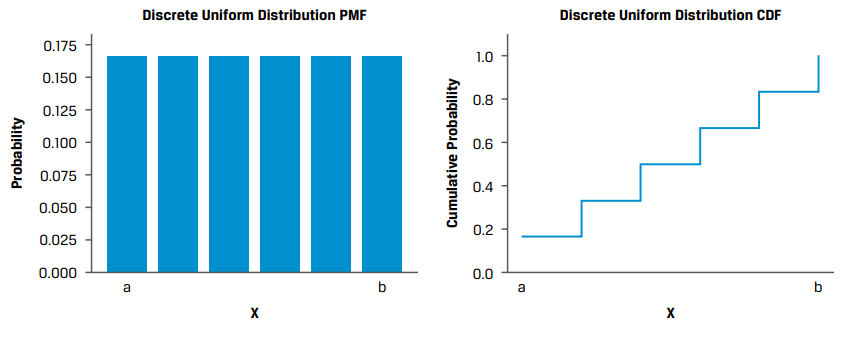
\includegraphics[width=0.85\linewidth]{002_figs/006_Module_6/exhibit_9.png}
	\caption{Discrete Uniform Distribution PMF and CDF}
	\label{fig:mod6_exhibit_9}
\end{figure}
\textcolor{blue}{\textit{Chứng minh công thức kỳ vọng, phương sai xem thêm phần (\ref{sec:Proof_Discrete_Uniform})}}

\subsubsection{Binomial Distribution}
The binomial distribution models the number of successes in a fixed number $n$ of independent Bernoulli trials, where each trial has a success probability $p$ and a failure probability $q = 1-p$.
The probability of observing exactly $x$ successes is:
\begin{equation}
	P(X=x) = \binom{n}{x} p^x (1-p)^{n-x}
	\label{eq:binomial_pmf_m6}
\end{equation}
The mean and variance are:
\begin{equation}
	\text{Mean: } \mu = n \times p
	\label{eq:binomial_mean_m6}
\end{equation}
\begin{equation}
	\text{Variance: } \sigma^2 = n \times p(1 - p)
	\label{eq:binomial_variance_m6}
\end{equation}

\textcolor{blue}{\textit{Chứng minh công thức PMF, kỳ vọng, phương sai xem thêm phần (\ref{sec:Proof_Binomial})}}

\begin{figure}[!htbp]
	\centering
	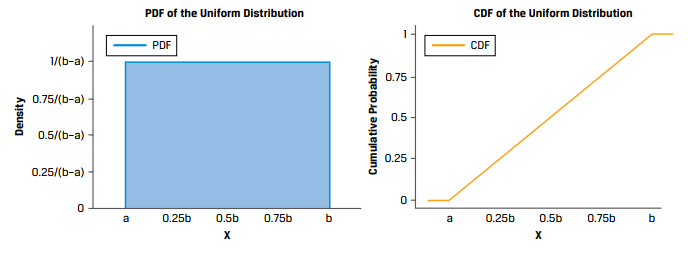
\includegraphics[width=0.95\linewidth]{002_figs/006_Module_6/exhibit_11.png}
	\caption{Binomial PMF and CDF Across Different Success Probabilities}
	\label{fig:mod6_exhibit_11}
\end{figure}

If $n$ is large, the binomial distribution can be approximated by a normal distribution:
\begin{equation}
	X \sim N(np, np(1-p))
	\label{eq:binomial_normal_approx_m6}
\end{equation}
This approximation is generally valid when both $np \ge 5$ and $n(1-p) \ge 5$.

\subsubsection{Poisson Distribution}
The Poisson distribution models the number of independent events occurring in a fixed interval of time or space at a constant average rate $\lambda$. The probability of observing $k$ events is:
\begin{equation}
	P(X=k) = \frac{\lambda^k e^{-\lambda}}{k!}
	\label{eq:poisson_pmf_m6}
\end{equation}
The mean and variance of a Poisson distribution are identical:
\begin{equation}
	\mu = \sigma^2 = \lambda
	\label{eq:poisson_moments_m6}
\end{equation}
Its skewness is $\frac{1}{\sqrt{\lambda}}$ and excess kurtosis is $\frac{1}{\lambda}$.

\textcolor{blue}{\textit{Phân phối Poisson được dùng để đếm số lần một sự kiện xảy ra trong một khoảng thời gian/không gian xác định (ví dụ: số cuộc gọi đến tổng đài mỗi giờ, số vụ vỡ nợ của doanh nghiệp trong một năm).
Đối với Binomial là tính xác suất thành công trong $n$ lần thử, Poisson là chia thời gian thành vô số khoảng nhỏ và đếm số lần sự kiện xảy ra trong mỗi khoảng.
Xác suất của sự kiện là $p=\frac{\lambda}{n}$ hay $\lambda=np$, khi $n$ lớn và $p$ nhỏ, phân phối Binomial tiệm cận với Poisson.}}

\textcolor{blue}{\textit{Chứng minh công thức PMF, kỳ vọng, phương sai xem thêm phần (\ref{sec:Proof_Poisson})}}

\begin{itemize}
	\item Probability of no default over time $t$: $P(\text{No default}) = e^{-\lambda t}$
	\item Probability of default over time $t$: $P(\text{Default}) = 1 - e^{-\lambda t}$
	\item Expected time to first default: $E[t_d] = \frac{1}{\lambda}$
\end{itemize}
In credit risk modeling, the Poisson distribution is widely used in \textbf{reduced-form models} where default is modeled as a random event governed by a hazard rate (default intensity) $\lambda$.

\textcolor{blue}{\textit{Ý nghĩa trong Quản trị Rủi ro Tín dụng: Giả sử một doanh nghiệp có xác suất vỡ nợ không đổi $\lambda$ mỗi năm. Phân phối Poisson cho phép tính xác suất để doanh nghiệp KHÔNG vỡ nợ sau thời gian $t$ là $e^{-\lambda t}$. Nếu một công ty có tỷ lệ vỡ nợ trung bình $\lambda = 2\%$ một năm ($\lambda = 0.02$), thì thời gian trung bình cho tới khi công ty này thực sự vỡ nợ là $E[t_d] = \frac{1}{0.02} = 50$ năm.}}

\begin{tcolorbox}[
	colback=gray!5!white,
	colframe=black!15!white,
	boxrule=0.5pt,
	arc=3pt,
	title=\textbf{Case Study: Predicting Corporate Default},
	coltitle=black,
	colbacktitle=black!5!white,
	before skip=6pt,
	after skip=6pt,
	breakable
]
Assume the hazard rate $\lambda$ for a corporate bond is $0.02$ per year.
\begin{itemize}
	\item Probability of default within 1 year: $P(\text{Default}) = 1 - e^{-0.02 \times 1} \approx 1.98\%$
	\item Probability of no default within 1 year: $P(\text{No default}) = e^{-0.02 \times 1} \approx 98.02\%$
	\item Expected time until first default: $E[t_d] = \frac{1}{0.02} = 50 \text{ years}$
\end{itemize}
\end{tcolorbox}

\begin{figure}[!htbp]
	\centering
	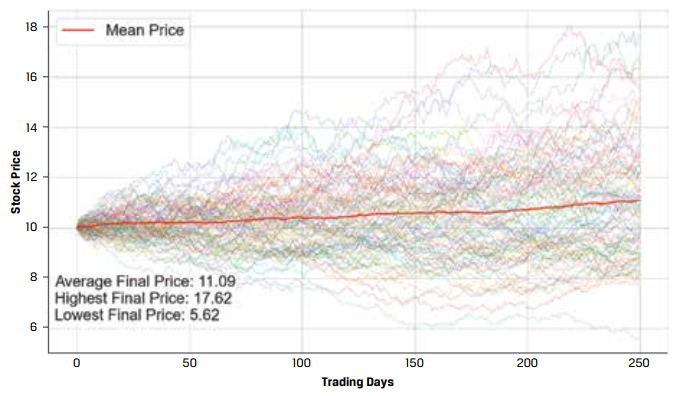
\includegraphics[width=0.95\linewidth]{002_figs/006_Module_6/exhibit_12.png}
	\caption{Poisson Distributions for Different Values of Lambda}
	\label{fig:mod6_exhibit_12}
\end{figure}

\subsection{Continuous Statistical Distributions}
	\label{subsec:Continuous Statistical Distributions}

\subsubsection{Continuous Uniform Distribution}
The continuous uniform distribution is defined over an interval $[a, b]$, where any value within this interval is equally likely to occur.
\begin{equation}
	\text{Mean: } \mu = \frac{a + b}{2}
	\label{eq:continuous_uniform_mean_m6}
\end{equation}
\begin{equation}
	\text{Variance: } \sigma^2 = \frac{(b - a)^2}{12}
	\label{eq:continuous_uniform_var_m6}
\end{equation}
Its skewness is $0$ and kurtosis is $1.8$.

\textcolor{blue}{\textit{Phân phối đều liên tục mô tả trường hợp một biến liên tục có khả năng xuất hiện bất kỳ giá trị nào trong khoảng $[a, b]$ với cơ hội như nhau. Mật độ xác suất $f(x)$ là một đường thẳng nằm ngang ở mức $\frac{1}{b-a}$. Do đó, diện tích dưới đường cong (chính là xác suất) trên bất kỳ phân đoạn nhỏ nào có độ dài $L$ luôn bằng $\frac{L}{b-a}$.}}

\textcolor{blue}{\textit{Chứng minh công thức kỳ vọng, phương sai xem thêm phần (\ref{sec:Proof_Continuous_Uniform})}}


\begin{figure}[!htbp]
	\centering
	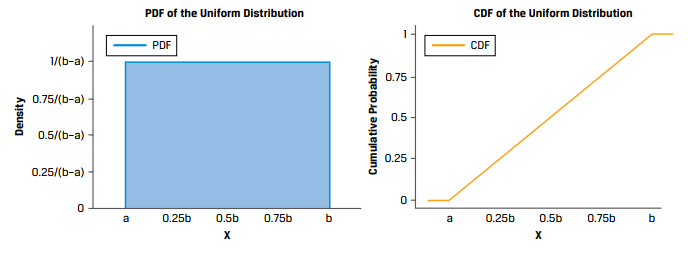
\includegraphics[width=0.85\linewidth]{002_figs/006_Module_6/exhibit_13.png}
	\caption{Continuous Uniform Probability Density between a and b}
	\label{fig:mod6_exhibit_13}
\end{figure}

Continuous uniform distributions are key to generating Monte Carlo simulations. To simulate any continuous distribution, we first draw random numbers from a standard uniform distribution $U \sim [0, 1]$ and then map them to the target distribution using the inverse CDF method.

\begin{tcolorbox}[
	colback=gray!5!white,
	colframe=black!15!white,
	boxrule=0.5pt,
	arc=3pt,
	title=\textbf{Case Study: Monte Carlo Simulation and Geometric Brownian Motion (GBM)},
	coltitle=black,
	colbacktitle=black!5!white,
	before skip=6pt,
	after skip=6pt,
	breakable
]
Stock price paths are often simulated using the GBM formula:
\[ S_t = S_0 e^{\left(\mu - \frac{\sigma^2}{2}\right)t + \sigma W_t} \]
where $\mu$ is drift, $\sigma$ is volatility, and $W_t$ is Brownian motion (normally distributed noise).
To simulate a single daily step ($t = 1/250$):
\begin{enumerate}
	\item Draw a uniform random value from $[0, 1]$, say $U = 0.07$.
	\item Convert it into a standard normal value: using the inverse standard normal CDF, $\Phi^{-1}(0.07) \approx -1.48$.
	\item Substitute $W_t = -1.48$ into the formula to compute the next stock price $S_1$.
\end{enumerate}
\end{tcolorbox}

% \begin{figure}[!htbp]
% 	\centering
% 	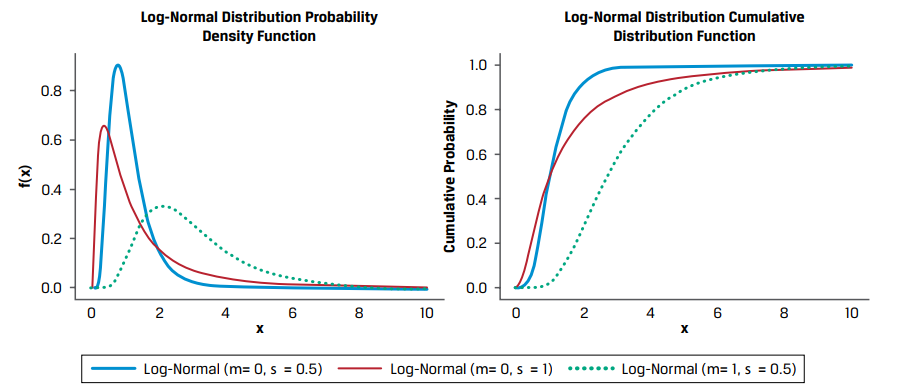
\includegraphics[width=0.85\linewidth]{002_figs/006_Module_6/exhibit_14.png}
% 	\caption{Monte Carlo Simulation Stock Price Paths}
% 	\label{fig:mod6_exhibit_14}
% \end{figure}

\subsubsection{Normal Distribution}
The normal distribution, or Gaussian distribution, is fully defined by its mean $\mu$ and variance $\sigma^2$, denoted as $N(\mu, \sigma^2)$.
It has a symmetrical bell shape where Mean = Median = Mode. Its skewness is $0$, kurtosis is $3$, and excess kurtosis is $0$.

\textcolor{blue}{\textit{Phân phối Chuẩn là phân phối quan trọng nhất trong tài chính học và thống kê nhờ Định lý Giới hạn Trung tâm (Central Limit Theorem). Đường cong mật độ PDF có dạng hình chuông đối xứng hoàn toàn qua giá trị trung bình $\mu$. Vì đối xứng nên các số đo xu hướng trung tâm gồm Kỳ vọng (Mean), Trung vị (Median) và Yếu vị (Mode) trùng nhau. Đặc điểm đặc trưng khác là Skewness = 0 và Kurtosis = 3 (Excess Kurtosis = 0).}}

\begin{figure}[!htbp]
	\centering
	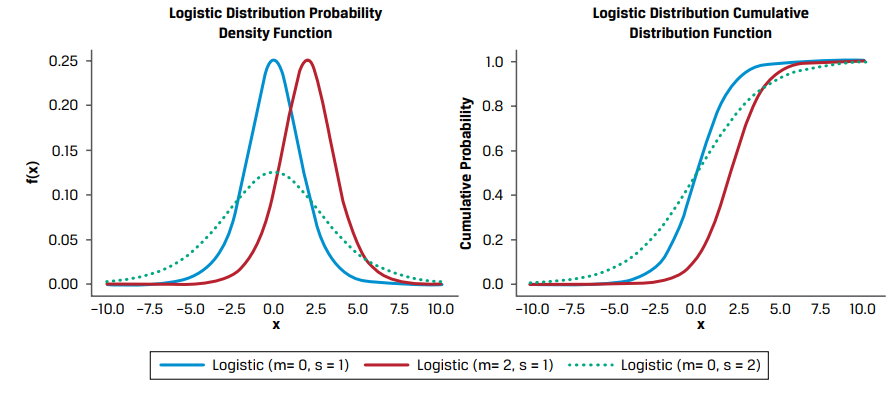
\includegraphics[width=0.85\linewidth]{002_figs/006_Module_6/exhibit_15.png}
	\caption{Standard Normal Distribution PDF and CDF}
	\label{fig:mod6_exhibit_15}
\end{figure}

A standard normal distribution has $\mu = 0$ and $\sigma^2 = 1$. Z-scores standardize any normal variable: $Z = \frac{X - \mu}{\sigma}$.
Key probability intervals (Empirical Rule):
\begin{itemize}
	\item $\mu \pm 1\sigma$ contains approximately $68\%$ of the observations.
	\item $\mu \pm 1.96\sigma$ contains approximately $95\%$ of the observations (often rounded to $\mu \pm 2\sigma$).
	\item $\mu \pm 2.58\sigma$ contains approximately $99\%$ of the observations.
\end{itemize}

\textcolor{blue}{\textit{Ý nghĩa của Z-score và Quy tắc thực nghiệm: Z-score đại diện cho khoảng cách từ biến $X$ tới trung bình tính theo số lần độ lệch chuẩn. Quy tắc thực nghiệm cho phép ta dự tính nhanh xác suất rơi vào các khoảng kỳ vọng: ví dụ có khoảng 95\% khả năng kết quả thực tế rơi trong khoảng $[-1.96\sigma, +1.96\sigma]$ xung quanh giá trị trung bình tổng thể.}}

\subsubsection{Log-Normal Distribution}
A random variable $Y$ is log-normally distributed if $X = \ln(Y)$ is normally distributed.
Because $Y = e^X$, log-normal variables can only take strictly positive values ($Y > 0$). The distribution is right-skewed.
% If $X \sim N(\mu_X, \sigma_X^2)$, the moments of $Y$ are:
% \begin{equation}
% 	\text{Mean: } \mu_Y = e^{\mu_X + \frac{\sigma_X^2}{2}}
% 	\label{eq:lognormal_mean_m6}
% \end{equation}
% \begin{equation}
% 	\text{Variance: } \sigma_Y^2 = (e^{\sigma_X^2} - 1) e^{2\mu_X + \sigma_X^2}
% 	\label{eq:lognormal_var_m6}
% \end{equation}

\textcolor{blue}{\textit{Biến $Y$ có phân phối Log-normal khi logarit tự nhiên của nó ($X = \ln(Y)$) có phân phối chuẩn. Do $Y = e^X$ và hàm mũ luôn dương nên biến log-normal bị chặn dưới bởi 0 ($Y > 0$). Phân phối này lệch phải (right-skewed) với phần đuôi kéo dài sang bên phải. Trong quản lý danh mục đầu tư, giá tài sản hoặc giá cổ phiếu luôn không thể âm nên được mô hình hóa bằng phân phối Log-normal. Ngược lại, tỷ suất sinh lời của tài sản (có thể là số âm) lại phù hợp với phân phối Chuẩn.}}

% \textcolor{blue}{\textit{Chứng minh phân phối Log-normal: Với $Y = e^X$ và $X \sim N(\mu_X, \sigma_X^2)$. Hàm sinh mô-men với $t=1$ cho $E[Y] = e^{\mu_X + \sigma_X^2/2}$. Đặt $t=2$ để tính $E[Y^2] = e^{2\mu_X + 2\sigma_X^2}$, suy ra phương sai $\text{Var}(Y) = (e^{\sigma_X^2} - 1) e^{2\mu_X + \sigma_X^2}$.}}

% \textcolor{blue}{\textit{Lưu ý: Giá cổ phiếu $\ge 0$ nên dùng phân phối Log-normal. Tỷ suất sinh lời có thể âm nên dùng phân phối Chuẩn. Log return có tính cộng dồn, giúp đơn giản hóa tính toán.}}

\begin{tcolorbox}[
	colback=gray!5!white,
	colframe=black!15!white,
	boxrule=0.5pt,
	arc=3pt,
	title=\textbf{Case Study: Modeling Asset Prices},
	coltitle=black,
	colbacktitle=black!5!white,
	before skip=6pt,
	after skip=6pt,
	breakable
]
Let $S_0 = 100$, logarithmic annual mean return $\mu = 8\%$, and volatility $\sigma = 20\%$. After $1$ year, the logarithmic price is:
\[ \ln(S_1) = \ln(S_0) + \left(\mu - \frac{\sigma^2}{2}\right) \times t = \ln(100) + \left(0.08 - \frac{0.04}{2}\right) \times 1 = 4.6652 \]
The expected future price is $S_1 = e^{4.6652} = 106.19$.
\end{tcolorbox}

\begin{figure}[!htbp]
	\centering
	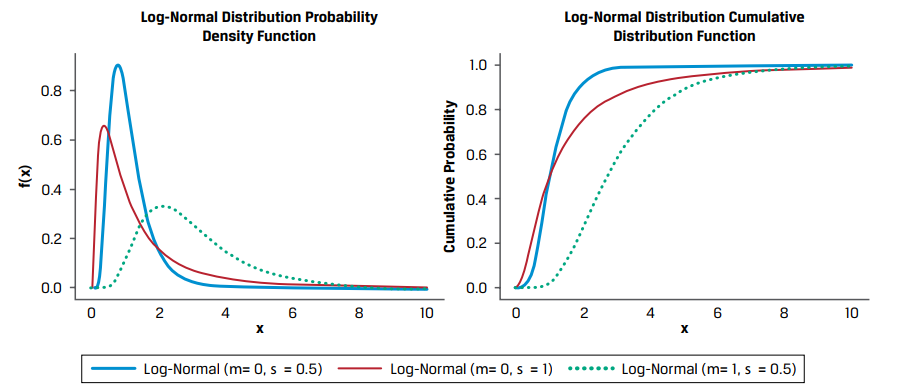
\includegraphics[width=0.85\linewidth]{002_figs/006_Module_6/exhibit_16.png}
	\caption{A Log-Normal Distribution Curve}
	\label{fig:mod6_exhibit_16_lognormal}
\end{figure}

\subsubsection{Logistic Distribution}
The logistic distribution is a continuous distribution defined by location $\mu$ and scale $s$. It resembles the normal distribution but has fatter tails.
\begin{equation}
	\text{Mean: } \mu_X = \mu
	\label{eq:logistic_mean_m6}
\end{equation}
\begin{equation}
	\text{Variance: } \sigma^2 = \frac{s^2 \pi^2}{3}
	\label{eq:logistic_variance_m6}
\end{equation}
Its skewness is $0$, kurtosis is $4.2$, and excess kurtosis is $1.2$.
The logistic distribution is widely used in logistic regression to predict binary outcomes in finance (e.g., probability of default).

\textcolor{blue}{\textit{Phân phối Logistic có hình dạng đối xứng hình chuông cực kỳ giống phân phối Chuẩn, nhưng phần đuôi của nó dày hơn (Fatter tails) - tức là khả năng xuất hiện các biến cố cực đoan cao hơn (Excess Kurtosis = 1.2 > 0). Phân phối này là nền tảng của mô hình Hồi quy Logistic (Logistic Regression) được dùng nhiều để dự đoán xác suất vỡ nợ tín dụng hoặc phân loại rủi ro (Default vs Non-default).}}

% \textcolor{blue}{\textit{Chứng minh phân phối Logistic: Với $X = \mu + s Z$ và $Z$ có CDF $F(z) = 1/(1+e^{-z})$. Do đối xứng, $E[X] = \mu$. Phương sai của $Z$ tính bằng tích phân Riemann-Zeta là $\pi^2/3$, do đó $\text{Var}(X) = s^2 \pi^2 / 3$.}}

\begin{figure}[!htbp]
	\centering
	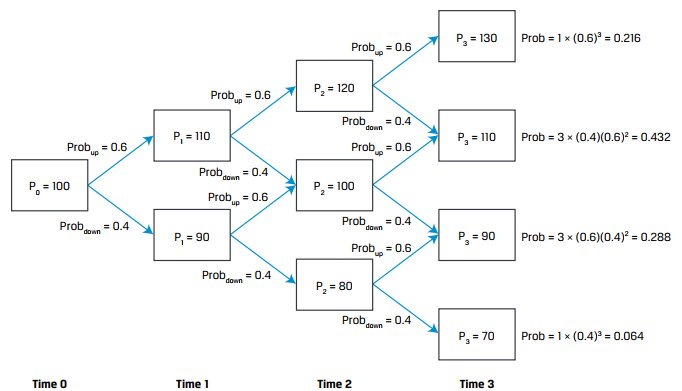
\includegraphics[width=0.85\linewidth]{002_figs/006_Module_6/exhibit_17.png}
	\caption{The PDF and CDF of Different Logistic Distributions}
	\label{fig:mod6_exhibit_17_logistic}
\end{figure}

\subsection{Practical Implementation}
	\label{subsec:Practical Implementation}

% Table~\ref{tab:moments_all_m6} summarizes the moments of all distributions covered in this module, and Table~\ref{tab:distribution_formulas_m6} shows their density/mass functions and cumulative distributions.

% \begin{table}[!htbp]
% \centering
% \renewcommand{\arraystretch}{1.8}
% \caption{The Four Statistical Moments of Distributions}
% \label{tab:moments_all_m6}
% \begin{tabular}{p{0.18\linewidth} p{0.18\linewidth} p{0.22\linewidth} p{0.15\linewidth} p{0.15\linewidth}}
% \toprule
% \textbf{Distribution} & \textbf{Mean} & \textbf{Variance} & \textbf{Skewness} & \textbf{Excess Kurtosis} \\
% \midrule
% Discrete Uniform & $\frac{a+b}{2}$ & $\frac{(b-a+1)^2-1}{12}$ & 0 & $-\frac{6(n^2+1)}{5(n^2-1)}$ \\
% Binomial & $np$ & $np(1-p)$ & $\frac{1-2p}{\sqrt{np(1-p)}}$ & $\frac{1-6p(1-p)}{np(1-p)}$ \\
% Poisson & $\lambda$ & $\lambda$ & $\frac{1}{\sqrt{\lambda}}$ & $\frac{1}{\lambda}$ \\
% Continuous Uniform & $\frac{a+b}{2}$ & $\frac{(b-a)^2}{12}$ & 0 & $-1.2$ \\
% Normal & $\mu$ & $\sigma^2$ & 0 & 0 \\
% Log-normal & $e^{\mu+\frac{\sigma^2}{2}}$ & $(e^{\sigma^2}-1)e^{2\mu+\sigma^2}$ & $>0$ & $>0$ \\
% Logistic & $\mu$ & $\frac{s^2\pi^2}{3}$ & 0 & 1.2 \\
% \bottomrule
% \end{tabular}
% \end{table}
% % Reference: CFA Curriculum 2027, Volume 1, Module 6, Page 289, Exhibit 18

% \begin{table}[!htbp]
% \centering
% \renewcommand{\arraystretch}{1.8}
% \caption{CDFs, PMFs, and PDFs for Statistical Distributions}
% \label{tab:distribution_formulas_m6}
% \begin{tabular}{p{0.18\linewidth} p{0.38\linewidth} p{0.38\linewidth}}
% \toprule
% \textbf{Distribution} & \textbf{PMF / PDF} & \textbf{CDF} \\
% \midrule
% Discrete Uniform & $\displaystyle \frac{1}{b-a+1}$ & $\displaystyle \frac{x-a+1}{b-a+1}$ \\
% Binomial & $\displaystyle \binom{n}{x} p^x (1-p)^{n-x}$ & $\displaystyle \sum_{i=0}^x \binom{n}{i} p^i (1-p)^{n-i}$ \\
% Poisson & $\displaystyle \frac{\lambda^x e^{-\lambda}}{x!}$ & $\displaystyle e^{-\lambda} \sum_{i=0}^x \frac{\lambda^i}{i!}$ \\
% Continuous Uniform & $\displaystyle \frac{1}{b-a}$ & $\displaystyle \frac{x-a}{b-a}$ \\
% Normal & $\displaystyle \frac{1}{\sigma\sqrt{2\pi}} e^{-\frac{1}{2}\left(\frac{x-\mu}{\sigma}\right)^2}$ & $\displaystyle \Phi\left(\frac{x-\mu}{\sigma}\right)$ \\
% Log-normal & $\displaystyle \frac{1}{x\sigma\sqrt{2\pi}} e^{-\frac{(\ln x - \mu)^2}{2\sigma^2}}$ & $\displaystyle \Phi\left(\frac{\ln x - \mu}{\sigma}\right)$ \\
% Logistic & $\displaystyle \frac{e^{-(x-\mu)/s}}{s\left(e^{-(x-\mu)/s}+1\right)^2}$ & $\displaystyle \frac{1}{e^{-(x-\mu)/s}+1}$ \\
% \bottomrule
% \end{tabular}
% \end{table}
% Reference: CFA Curriculum 2027, Volume 1, Module 6, Page 290, Exhibit 19

Table~\ref{tab:excel_formulas_m6} summarizes the Excel and Google Sheets formulas used to compute these distributions in practice.

\begin{table}[!htbp]
\centering
\renewcommand{\arraystretch}{1.5}
\caption{Statistical Distribution Functions in Excel and Google Sheets}
\label{tab:excel_formulas_m6}
\begin{tabular}{p{0.28\linewidth} p{0.33\linewidth} p{0.33\linewidth}}
\toprule
\textbf{Distribution Function} & \textbf{Excel Formula} & \textbf{Google Sheets Formula} \\
\midrule
Uniform CDF & \texttt{BETA.DIST((x-a)/(b-a),1,1,TRUE)} & \texttt{BETA.DIST((x-a)/(b-a),1,1,TRUE)} \\
Uniform Random Draw & \texttt{=RAND()*(b-a)+a} & \texttt{=RAND()*(b-a)+a} \\
Binomial PMF & \texttt{=BINOM.DIST(x, n, p, FALSE)} & \texttt{=BINOM.DIST(x, n, p, FALSE)} \\
Binomial CDF & \texttt{=BINOM.DIST(x, n, p, TRUE)} & \texttt{=BINOM.DIST(x, n, p, TRUE)} \\
Poisson PMF & \texttt{=POISSON.DIST(x, lambda, FALSE)} & \texttt{=POISSON.DIST(x, lambda, FALSE)} \\
Normal PDF & \texttt{=NORM.DIST(x, mean, sd, FALSE)} & \texttt{=NORM.DIST(x, mean, sd, FALSE)} \\
Normal Random Draw & \texttt{=NORM.INV(RAND(), mean, sd)} & \texttt{=NORMINV(RAND(), mean, sd)} \\
Log-normal CDF & \texttt{=LOGNORM.DIST(x, mean, sd, TRUE)} & \texttt{=LOGNORM.DIST(x, mean, sd, TRUE)} \\
\bottomrule
\end{tabular}
\end{table}
% Reference: CFA Curriculum 2027, Volume 1, Module 6, Page 290, Exhibit 20

\section{Conditional Expectations, Variances, and Covariances}
\label{sec:Conditional Expectations, Variances, and Covariances}
\begin{center}
\begin{tabular}{p{0.06\linewidth} | p{0.88\linewidth}}
	c & calculate, interpret, and evaluate conditional expectations, variances, and covariances \\
\end{tabular}
\end{center}

\subsection{Joint Distributions of Random Variables}
	\label{subsec:Joint Distributions of Random Variables}
Joint distributions allow for examining the simultaneous distribution of two random variables. The bivariate cumulative distribution function (CDF) is defined as:
\begin{equation}
	F_{12}(x_1, x_2) = P(X_1 \le x_1, X_2 \le x_2)
	\label{eq:joint_cdf_m6}
\end{equation}
For continuous variables, the joint CDF is obtained by integrating the joint PDF $f_{12}(u_1, u_2)$:
\begin{equation}
	F_{12}(x_1, x_2) = \int_{-\infty}^{x_1} \int_{-\infty}^{x_2} f_{12}(u_1, u_2) du_1 du_2
	\label{eq:joint_cdf_integral_m6}
\end{equation}
If the variables are independent:
\begin{equation}
	f_{12}(u_1, u_2) = f_1(u_1) \times f_2(u_2)
	\label{eq:joint_pdf_independent_m6}
\end{equation}

\begin{figure}[!htbp]
	\centering
	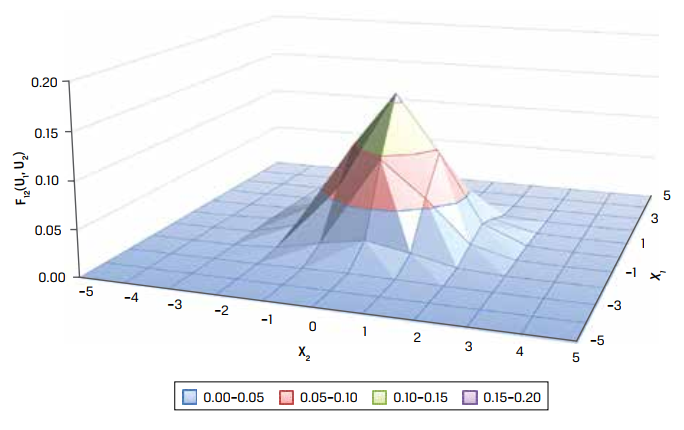
\includegraphics[width=0.85\linewidth]{002_figs/006_Module_6/exhibit_21.png}
	\caption{Joint Probability Density Surface Plot}
	\label{fig:mod6_exhibit_21}
\end{figure}

The \textbf{marginal density} is the probability distribution of a single variable within a multivariate distribution. It is obtained by integrating out the other variables:
\begin{equation}
	f_{X_1}(x_1) = \int_{-\infty}^{\infty} f_{X_1 X_2}(x_1, u_2) du_2
	\label{eq:marginal_density_m6}
\end{equation}

For discrete variables, joint and marginal distributions are summarized in contingency tables.

\begin{tcolorbox}[
	colback=gray!5!white,
	colframe=black!15!white,
	boxrule=0.5pt,
	arc=3pt,
	title=\textbf{Case Study: Stock Market Returns and Technology Companies},
	coltitle=black,
	colbacktitle=black!5!white,
	before skip=6pt,
	after skip=6pt,
	breakable
]
An index consists of $500$ firms, $100$ of which are technology firms.
Among the $100$ technology firms, $60$ had returns $> 10\%$ and $40$ had returns $\le 10\%$.
Among the $400$ non-tech firms, $100$ had returns $> 10\%$ and $300$ had returns $\le 10\%$.
Table~\ref{tab:contingency_tech_m6} displays these frequencies.
\end{tcolorbox}

\begin{table}[!htbp]
\centering
\caption{Returns for Technology and Non-Technology Firms}
\label{tab:contingency_tech_m6}
\begin{tabular}{p{0.25\linewidth} p{0.25\linewidth} p{0.20\linewidth} p{0.15\linewidth}}
\toprule
\textbf{Rate of Return} $R$ & \textbf{Non-Technology} & \textbf{Technology} & \textbf{Total} \\
\midrule
$R > 10\%$  & 100 & 60  & 160 \\
$R \le 10\%$ & 300 & 40  & 340 \\
\midrule
\textbf{Total} & \textbf{400} & \textbf{100} & \textbf{500} \\
\bottomrule
\end{tabular}
\end{table}
% Reference: CFA Curriculum 2027, Volume 1, Module 6, Page 295, Exhibit 22

\subsection{Conditional Expectations}
	\label{subsec:Conditional Expectations}
The conditional expectation $E[X | Y=y]$ is the expected value of $X$ given that $Y$ takes on the value $y$:
\begin{equation}
	\text{Discrete: } E[X|Y=y] = \sum_x x P(X=x | Y=y)
	\label{eq:discrete_cond_mean_m6}
\end{equation}
\begin{equation}
	\text{Continuous: } E[X|Y=y] = \int x f_{X|Y}(x|y) dx
	\label{eq:continuous_cond_mean_m6}
\end{equation}
The expected conditional variance is:
\begin{equation}
	\text{Var}(X | Y=y) = E[X^2 | Y=y] - (E[X | Y=y])^2
	\label{eq:conditional_variance_m6}
\end{equation}

% \textcolor{blue}{\textit{Kỳ vọng có điều kiện $E[X|Y=y]$ là giá trị trung bình của biến $X$ khi đã biết trước thông tin $Y$ nhận một giá trị cụ thể $y$. Ví dụ: Xác suất vỡ nợ trung bình của các doanh nghiệp là 2\% (kỳ vọng vô điều kiện), nhưng nếu biết nền kinh tế đang suy thoái sâu (thông tin điều kiện), xác suất vỡ nợ trung bình có thể tăng lên mức 15\% (kỳ vọng có điều kiện). Phương sai có điều kiện $\text{Var}(X|Y=y)$ đo lường rủi ro của biến $X$ trong bối cảnh cụ thể của điều kiện $Y=y$.}}

The \textbf{Total Probability Rule for Expected Value} states:
\begin{equation}
	E[X] = \sum_{i=1}^n E[X | S_i] \times P(S_i)
	\label{eq:total_prob_rule_expectation_m6}
\end{equation}
where $S_1, S_2, \dots, S_n$ are mutually exclusive and exhaustive scenarios.

% \textcolor{blue}{\textit{Công thức kỳ vọng toàn phần cho biết kỳ vọng chung của một biến số bằng trung bình trọng số của các kỳ vọng có điều kiện trong từng kịch bản có thể xảy ra, với trọng số chính là xác suất xảy ra kịch bản đó. Ví dụ, để tính tỷ suất sinh lời kỳ vọng năm tới của cổ phiếu ($E[R]$), ta tính tỷ suất sinh lời kỳ vọng trong 3 kịch bản: Tăng trưởng ($E[R|\text{Expansion}]$), Bình thường ($E[R|\text{Normal}]$), và Suy thoái ($E[R|\text{Recession}]$) rồi nhân với xác suất tương ứng của từng kịch bản đó rồi cộng lại.}}

\begin{tcolorbox}[
	colback=gray!5!white,
	colframe=black!15!white,
	boxrule=0.5pt,
	arc=3pt,
	title=\textbf{Case Study: Scenario Expected Returns and Variances},
	coltitle=black,
	colbacktitle=black!5!white,
	before skip=6pt,
	after skip=6pt,
	breakable
]
An analyst estimates portfolio return forecasts across three equally likely economic scenarios (Depression, Recession, and Expansion, each with probability $P = 1/3$):
\begin{itemize}
	\item \textbf{Depression}: $-25\%$ return (prob $50\%$), $-10\%$ return (prob $25\%$), $-5\%$ return (prob $15\%$), $0\%$ return (prob $10\%$).
	\item \textbf{Recession}: $-5\%$ return (prob $30\%$), $0\%$ return (prob $30\%$), $5\%$ return (prob $30\%$), $15\%$ return (prob $10\%$).
	\item \textbf{Expansion}: $50\%$ return (prob $40\%$), $10\%$ return (prob $25\%$), $15\%$ return (prob $25\%$), $25\%$ return (prob $10\%$).
\end{itemize}
Conditional expected returns and variances are calculated as:
\begin{align*}
	E[R|\text{Depression}] &= 0.50(-0.25) + 0.25(-0.10) + 0.15(-0.05) + 0.10(0) = -15.75\% \\
	\text{Var}[R|\text{Depression}] &= 0.50(-0.25 - (-0.1575))^2 + 0.25(-0.10 - (-0.1575))^2 \\
	&\quad + 0.15(-0.05 - (-0.1575))^2 + 0.10(0 - (-0.1575))^2 \\
	&\approx 0.009319 \\[1ex]
	E[R|\text{Recession}] &= 0.30(-0.05) + 0.30(0) + 0.30(0.05) + 0.10(0.15) = 1.50\% \\
	\text{Var}[R|\text{Recession}] &= 0.30(-0.05 - 0.015)^2 + 0.30(0 - 0.015)^2 \\
	&\quad + 0.30(0.05 - 0.015)^2 + 0.10(0.15 - 0.015)^2 \\
	&\approx 0.003525 \\[1ex]
	E[R|\text{Expansion}] &= 0.40(0.50) + 0.25(0.10) + 0.25(0.15) + 0.10(0.25) = 28.75\% \\
	\text{Var}[R|\text{Expansion}] &= 0.40(0.50 - 0.2875)^2 + 0.25(0.10 - 0.2875)^2 \\
	&\quad + 0.25(0.15 - 0.2875)^2 + 0.10(0.25 - 0.2875)^2 \\
	&\approx 0.031719
\end{align*}
If scenarios are equally likely, the unconditional expected return is:
\[ E[R] = \frac{-15.75\% + 1.50\% + 28.75\%}{3} = 4.833\% \]
The unconditional variance is computed using the Law of Total Variance:
\begin{equation}
	\text{Var}(R) = E[\text{Var}(R|S)] + \text{Var}(E[R|S])
	\label{eq:law_of_total_variance_example}
\end{equation}
where:
\[
E[\text{Var}(R|S)] = \frac{0.009319 + 0.003525 + 0.031719}{3} = 0.014854 \text{ (kỳ vọng của các phương sai có điều kiện)}
\]
\begin{align*}
\text{Var}(E[R|S]) &= \frac{1}{3}(-0.1575 - 0.048333)^2 + \frac{1}{3}(0.015 - 0.048333)^2 + \frac{1}{3}(0.2875 - 0.048333)^2 \\
&= 0.033560 \text{ (phương sai của các kỳ vọng có điều kiện)}
\end{align*}

Do đó, phương sai vô điều kiện của danh mục là:
\[ \text{Var}(R) = 0.014854 + 0.033560 = 0.048414 \text{ (hay } 4.84\% \text{)} \]

\vspace{0.5em}
\textcolor{blue}{\textit{\textbf{Đính chính Errata trong sách CFA Curriculum 2027 gốc:}}}

\textcolor{blue}{\textit{1. \textbf{Phát hiện lỗi:} Trong giáo trình CFA Curriculum, phương sai của các kỳ vọng có điều kiện $\text{Var}(E[R|S])$ đã bỏ quên dấu âm của kịch bản Depression (nhập nhầm $\mathbf{+0.1575}$ thay vì $\mathbf{-0.1575}$ trong phép trừ với $E[R] = 0.048333$), dẫn đến kết quả bị sai thành:}}
{\color{blue}
\begin{align*}
\text{Var}(E[R|S])_{\text{CFA}} &= \frac{1}{3}(\mathbf{+0.1575} - 0.048333)^2 + \frac{1}{3}(0.015 - 0.048333)^2 \\
&\quad + \frac{1}{3}(0.2875 - 0.048333)^2 = 0.02341 \approx \mathbf{0.0234} \quad (\mathbf{2.34\%})
\end{align*}
}

\textcolor{blue}{\textit{2. \textbf{Phép tính chuẩn xác (giữ đúng dấu âm $-15.75\%$):}}}
{\color{blue}
\begin{align*}
\text{Var}(E[R|S])_{\text{Chuẩn}} &= \frac{1}{3}(\mathbf{-0.1575} - 0.048333)^2 + \frac{1}{3}(0.015 - 0.048333)^2 \\
&\quad + \frac{1}{3}(0.2875 - 0.048333)^2 = 0.033560 \quad (\mathbf{3.36\%})
\end{align*}
}

\textcolor{blue}{\textit{3. \textbf{Phương sai vô điều kiện theo Law of Total Variance:}}}
\[
\textcolor{blue}{\text{Var}(R) = E[\text{Var}(R|S)] + \text{Var}(E[R|S]) = 0.014854 + 0.033560 = \mathbf{0.048414} \quad (\mathbf{4.84\%})}
\]
\textcolor{blue}{\textit{Xem thêm về Law of Total Variance tại phần (\ref{sec:Law_of_Total_Variance})}}
\end{tcolorbox}

\subsection{Conditional Means, Variances, and Covariances}
	\label{subsec:Conditional Means, Variances, and Covariances}
Incorporating conditioning information updates expected values:
\begin{itemize}
	\item \textbf{Conditional Mean:} $E[X|S] = \sum_{i=1}^n x_i P(X_i|S)$
	\item \textbf{Conditional Variance:} $\text{Var}(X|S) = E[(X - E[X|S])^2 | S]$
	\item \textbf{Conditional Covariance:}
	\begin{equation}
		\text{Cov}(X, Y | S) = E[(X - E[X|S])(Y - E[Y|S]) | S]
		\label{eq:conditional_covariance_formula_m6}
	\end{equation}
\end{itemize}

% \textcolor{blue}{\textit{Giải thích trực quan: Khi có thông tin mới $S$, cả kỳ vọng, phương sai và hiệp phương sai của các tài sản đều được cập nhật (updated). Ví dụ, trong điều kiện thị trường bình thường ($S = \text{Bình thường}$), cổ phiếu và vàng có thể có tương quan rất thấp hoặc ngược chiều ($\text{Cov}(X,Y|S) < 0$). Tuy nhiên, trong điều kiện khủng hoảng tài chính toàn cầu ($S = \text{Khủng hoảng}$), các nhà đầu tư tháo chạy khỏi mọi tài sản rủi ro để nắm giữ tiền mặt, khiến hiệp phương sai có điều kiện giữa nhiều loại tài sản đột ngột tăng mạnh cùng chiều.}}

\begin{tcolorbox}[
	colback=gray!5!white,
	colframe=black!15!white,
	boxrule=0.5pt,
	arc=3pt,
	title=\textbf{Case Study: Three-Period Asset Price Evolution},
	coltitle=black,
	colbacktitle=black!5!white,
	before skip=6pt,
	after skip=6pt,
	breakable
]
Let $P_0 = 100$. Each period, the price rises by $10$ with probability $0.60$ or falls by $10$ with probability $0.40$. At Time 3, possible outcomes follow a binomial tree (Exhibit~\ref{fig:mod6_exhibit_25}):
\begin{itemize}
	\item $P_3 = 130$ (prob $0.6^3 = 0.216$)
	\item $P_3 = 110$ (prob $3 \times 0.6^2 \times 0.4 = 0.432$)
	\item $P_3 = 90$ (prob $3 \times 0.6 \times 0.4^2 = 0.288$)
	\item $P_3 = 70$ (prob $0.4^3 = 0.064$)
\end{itemize}
The unconditional price expectation at Time 3 is:
\[ E[P_3] = 130(0.216) + 110(0.432) + 90(0.288) + 70(0.064) = 106 \]
The unconditional variance is:
\[ \text{Var}(P_3) = E[P_3^2] - (E[P_3])^2 = 11,524 - 106^2 = 288 \]

Suppose at Time 1, the price is observed to be $110$ ($P_1 = 110$, Exhibit~\ref{fig:mod6_exhibit_26}). The conditional probabilities for Time 3 update to:
\begin{itemize}
	\item $P_3 = 130$ (prob $0.6^2 = 0.36$)
	\item $P_3 = 110$ (prob $2 \times 0.6 \times 0.4 = 0.48$)
	\item $P_3 = 90$ (prob $0.4^2 = 0.16$)
\end{itemize}
The conditional expectation is:
\[ E[P_3|P_1=110] = 130(0.36) + 110(0.48) + 90(0.16) = 114 \]
The conditional variance is:
\[ \text{Var}(P_3|P_1=110) = E[P_3^2|P_1=110] - E[P_3|P_1=110]^2 = 15,568 - 114^2 = 192 \]

Suppose at Time 2, the price is $100$ ($P_2 = 100$, Exhibit~\ref{fig:mod6_exhibit_27}). The conditional statistics update to:
\[ E[P_3|P_2=100] = 110(0.60) + 90(0.40) = 102 \]
\[ \text{Var}(P_3|P_2=100) = (110^2 \times 0.60 + 90^2 \times 0.40) - 102^2 = 96 \]

Table~\ref{tab:binomial_cond_summary_m6} summarizes the updates:
\end{tcolorbox}

\begin{figure}[!htbp]
	\centering
	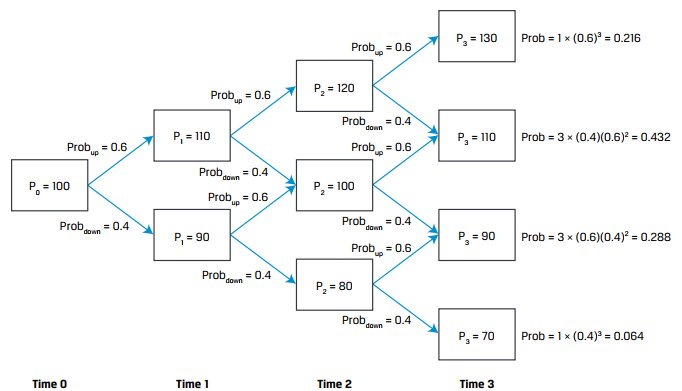
\includegraphics[width=0.75\linewidth]{002_figs/006_Module_6/exhibit_25.png}
	\caption{Potential Asset Price Evolution over Three Periods}
	\label{fig:mod6_exhibit_25}
\end{figure}

\begin{figure}[!htbp]
	\centering
	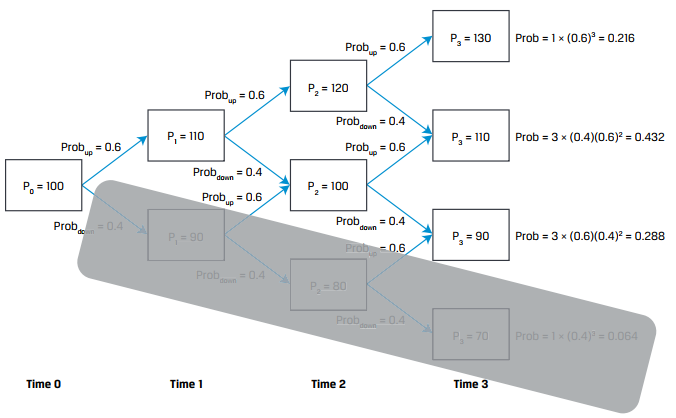
\includegraphics[width=0.75\linewidth]{002_figs/006_Module_6/exhibit_26.png}
	\caption{Price Evolution Given Time 1 Outcome $P_1 = 110$}
	\label{fig:mod6_exhibit_26}
\end{figure}

\begin{figure}[!htbp]
	\centering
	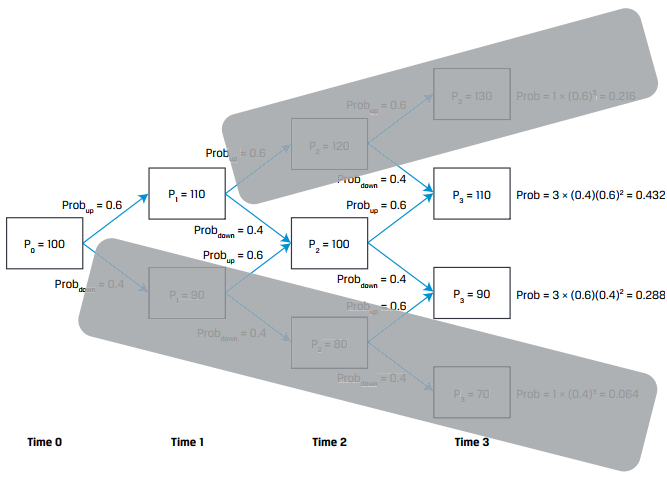
\includegraphics[width=0.75\linewidth]{002_figs/006_Module_6/exhibit_27.png}
	\caption{Price Evolution Given Time 2 Outcome $P_2 = 100$}
	\label{fig:mod6_exhibit_27}
\end{figure}

\begin{table}[!htbp]
\centering
\caption{Expectation and Variance Under Different Conditions}
\label{tab:binomial_cond_summary_m6}
\begin{tabular}{p{0.35\linewidth} p{0.25\linewidth} p{0.25\linewidth}}
\toprule
\textbf{Conditionality} & \textbf{Expected Price} & \textbf{Variance} \\
\midrule
Unconditional & 106 & 288 \\
Conditional on $P_1 = 110$ & 114 & 192 \\
Conditional on $P_2 = 100$ & 102 & 96 \\
\bottomrule
\end{tabular}
\end{table}

\section{Bayesian Updating}
\label{sec:Bayesian Updating}
\begin{center}
\begin{tabular}{p{0.06\linewidth} | p{0.88\linewidth}}
	d & formulate investment problems through Bayesian updating \\
\end{tabular}
\end{center}

Bayes' theorem provides a formal framework for updating the probability of a hypothesis (prior probability) in light of additional data or evidence to form an updated probability (posterior probability).
\begin{itemize}
	\item \textbf{A Priori Probability (Prior):} The probability of an event formulated before new data is considered.
	\item \textbf{A Posteriori Probability (Posterior):} The updated probability of the event after incorporating new observations.
\end{itemize}

Bayes' formula is stated as:
\begin{equation}
	P(A|B) = \frac{P(B|A) \times P(A)}{P(B)}
	\label{eq:bayes_formula_m6}
\end{equation}
where:
\begin{itemize}
	\item $P(A|B)$ is the posterior probability of $A$ occurring given $B$ is true.
	\item $P(B|A)$ is the likelihood of observing $B$ given $A$ is true.
	\item $P(A)$ is the prior probability of $A$.
	\item $P(B)$ is the marginal probability of observing $B$, computed using the total probability rule:
	\begin{equation}
		P(B) = \sum_i P(B|A_i) \times P(A_i)
		\label{eq:total_prob_denominator_m6}
	\end{equation}
\end{itemize}
\textcolor{blue}{\textit{Ý nghĩa thực tế: Định lý Bayes giúp cập nhật nhận định ban đầu của chúng ta khi có thêm thông tin mới.}}

\textcolor{blue}{\textit{Quy trình 3 bước tính toán xác suất cập nhật Bayes:}}
\begin{enumerate}
	\item[] \textcolor{blue}{\textit{\textbf{Bước 1 - Xác định thông tin ban đầu (Prior \& Likelihood):} Xác định xác suất tiên nghiệm của các kịch bản $P(A_i)$ và xác suất có điều kiện xảy ra thông tin mới trong từng kịch bản $P(B|A_i)$.}}
	\item[] \textcolor{blue}{\textit{\textbf{Bước 2 - Tính xác suất toàn phần (Total Probability):} Tính tổng xác suất xảy ra thông tin mới $P(B) = \sum P(B|A_i) P(A_i)$. Đây chính là mẫu số trong công thức Bayes.}}
	\item[] \textcolor{blue}{\textit{\textbf{Bước 3 - Tính xác suất hậu nghiệm (Posterior):} Lấy xác suất đồng thời của kịch bản mục tiêu chia cho xác suất toàn phần: $P(A_i|B) = \frac{P(B|A_i) P(A_i)}{P(B)}$.}}
\end{enumerate}

\begin{tcolorbox}[
	colback=gray!5!white,
	colframe=black!15!white,
	boxrule=0.5pt,
	arc=3pt,
	title=\textbf{Case Study: Technology Companies and Stock Returns},
	coltitle=black,
	colbacktitle=black!5!white,
	before skip=6pt,
	after skip=6pt,
	breakable
]
Using the contingency table for technology firms in Table~\ref{tab:contingency_tech_m6}, we calculate:
\begin{itemize}
	\item $P(\text{Tech}) = 0.20$ and $P(\text{Non-tech}) = 0.80$
	\item $P(R > 10\% | \text{Tech}) = 0.60$ and $P(R > 10\% | \text{Non-tech}) = 0.25$
\end{itemize}
The overall probability of a firm having a return $R > 10\%$ is:
\[ P(R > 10\%) = (0.60 \times 0.20) + (0.25 \times 0.80) = 0.32 \]
Using Bayes' formula, the probability that a firm is a technology company given its return exceeds $10\%$ is:
\[ P(\text{Tech} | R > 10\%) = \frac{P(R > 10\% | \text{Tech}) \times P(\text{Tech})}{P(R > 10\%)} = \frac{0.60 \times 0.20}{0.32} = 37.5\% \]
This represents an increase from the unconditional prior probability of $20\%$.
\end{tcolorbox}

\begin{tcolorbox}[
	colback=gray!5!white,
	colframe=black!15!white,
	boxrule=0.5pt,
	arc=3pt,
	title=\textbf{Case Study: Sustainability Investments and Earnings Expectations},
	coltitle=black,
	colbacktitle=black!5!white,
	before skip=6pt,
	after skip=6pt,
	breakable
]
EcoMed A/S will release its annual earnings next week. Prior probabilities for consensus EPS outcomes are:
\begin{itemize}
	\item $P(\text{Exceeded Consensus}) = 0.45$
	\item $P(\text{Met Consensus}) = 0.30$
	\item $P(\text{Fell Short}) = 0.25$
\end{itemize}
Before the release, EcoMed announces expanding sustainable practices. The likelihood of this announcement under each earnings scenario is estimated as:
\begin{itemize}
	\item $P(\text{Sustainability Announcement} | \text{Exceeded}) = 0.75$
	\item $P(\text{Sustainability Announcement} | \text{Met}) = 0.20$
	\item $P(\text{Sustainability Announcement} | \text{Fell Short}) = 0.05$
\end{itemize}
First, we find the unconditional probability of the sustainability announcement:
\[ P(\text{Sustainability}) = (0.75 \times 0.45) + (0.20 \times 0.30) + (0.05 \times 0.25) = 0.41 \]
We update the probabilities using Bayes' formula:
\begin{align*}
	P(\text{Exceeded} | \text{Sustainability}) &= \frac{0.75 \times 0.45}{0.41} = 82.32\% \\
	P(\text{Met} | \text{Sustainability}) &= \frac{0.20 \times 0.30}{0.41} = 14.63\% \\
	P(\text{Fell Short} | \text{Sustainability}) &= \frac{0.05 \times 0.25}{0.41} = 3.05\%
\end{align*}
Note that the updated posterior probabilities sum to exactly $1.0000$:
\[ 0.8232 + 0.1463 + 0.0305 = 1.0000 \]

% \textcolor{blue}{\textit{Bảng tính toán cập nhật Bayes hệ thống (Phương pháp khuyên dùng khi đi thi):}}
\begin{center}
\resizebox{\linewidth}{!}{%
\begin{tabular}{l c c c c}
\toprule
\textbf{Kịch bản ($A_i$)} & \textbf{Prior} $P(A_i)$ & \textbf{Likelihood} $P(B|A_i)$ & \textbf{Joint Probability} $P(B \cap A_i)$ & \textbf{Posterior} $P(A_i|B)$ \\
\midrule
Exceeded Consensus & 0.45 & 0.75 & 0.3375 & 82.32\% \\
Met Consensus      & 0.30 & 0.20 & 0.0600 & 14.63\% \\
Fell Short         & 0.25 & 0.05 & 0.0125 & 3.05\% \\
\midrule
\textbf{Tổng}      & \textbf{1.00} & & \textbf{$P(\text{Sustainability}) = 0.4100$} & \textbf{100.00\%} \\
\bottomrule
\end{tabular}%
}
\end{center}
\end{tcolorbox}


% \section{Practice Problems and Solutions}
% \label{sec:Practice_Problems_Module_6}
% \textcolor{blue}{\textit{Các bài tập ôn tập kèm Lời giải của Module 6 đã được chuyển về Chương 14 (Bài tập ôn tập và Lời giải) ở cuối bản PDF để tiện tra cứu tập trung. Xem bài tập và lời giải tại trang \pageref{sec:app_Problems_M6}.}}
